% !TEX root = Dokumentation_SysSpec.tex
\subsection{Modelle und Sichten}

\subsubsection{Kontextdiagramm}
todo bla
\begin{figure}[H]
	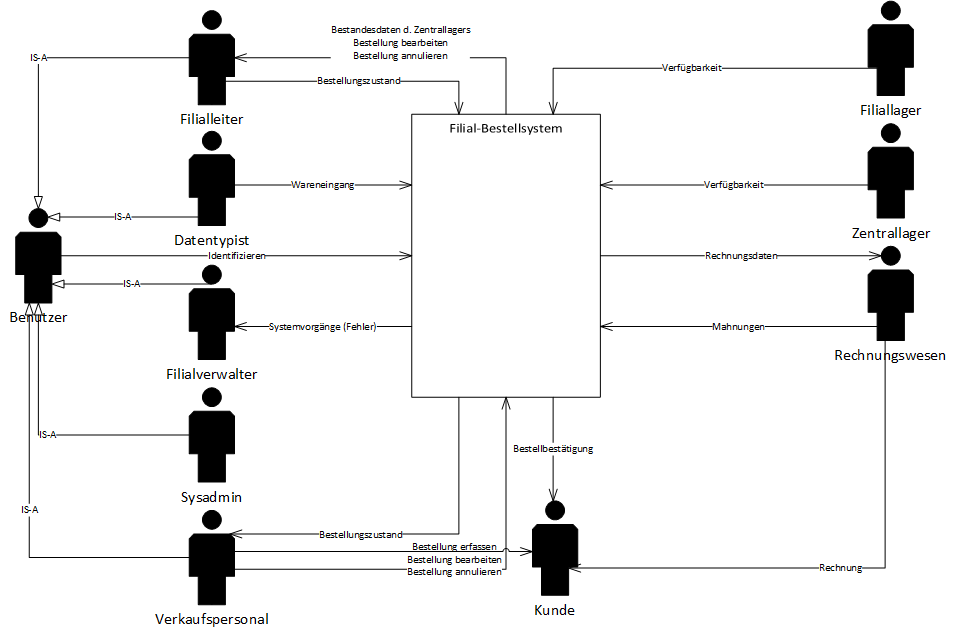
\includegraphics[width=1.0\linewidth]{Images/kontextdiagram}
	\caption{Kontextdiagram}
	\label{fig:kontextdiagram}
\end{figure}

\subsubsection{Layer-Architektur}
TODO Übersichsgrafik importieren und erläutern

\subsubsection{Client-Layer}
Der Client-Layer ist in JavaFX implementiert und verwendet das MVC-Architektur-Pattern. Zur Gestaltung der Oberfläche wurde ein 3rd Party Tool eingesetzt, um die graphische Gestaltung zu vereinfachen.
\begin{itemize}
\item Scene Builder by Gluon: Basiert auf der von Oracle entwickelten JavaFX-Distribution, und erstellt ein passendes FXML-Dokument für die Einbindung der graphischen Oberfläche, inklusive Verlinkung und definition der Event-Handler. 
\end{itemize}
\begin{figure}[H]
	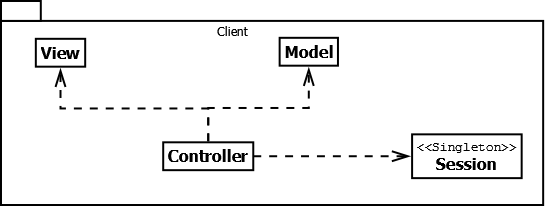
\includegraphics[width=1.0\linewidth]{Images/ClientLayer-Architektur}
	\caption{Architektur des Clientlayer}
	\label{fig:clientlayer-architektur}
\end{figure}

\textbf{View}: Die View ist dafür verantwortlich, dass die angezeigte Oberfläche korrekt geladen ist.

\textbf{Controller}: Die Controller binden die FXML-Dokumente ein. Die Controller registrieren ausgelöste Events und steuern die durchzufürenden Aktionen, wie Datenabfragen vom Business-Layer durch.

\textbf{Model}: Im Model befinden sich die im GUI angezeigten Datenwerte, und sind bereits durch die Verwendung von Property-Klassen als Observable-Objekte abgespeichert.

\textbf{Session}: Die Session enthält die User-Informationen. Die Session-Informationen werden bei Aktionen mitgesendet, um unauthorisierte Aufrufe zu unterbinden.

\subsubsection{Remote-Layer}
\subsubsection{Business-Layer}
\subsubsection{Data-Layer}
\subsubsection{Model-Layer}

\subsubsection{UML-Klassendiagramme}



\subsubsection{Sequenzdiagramme}
todo


\subsection{Entwurfsentscheid}
Im Rahmen der Architekturausarbeitung wurden folgende Entwurfsentscheide gefällt:
\begin{itemize}
	\item Für Testzwecke und statische Datenstrukturen werden teilweise Stubs eingesetzt. Beispielsweise sind die Zuweisung Benutzerrollen zu deren Berechtigungen bis Release 1.0 als Stub abgebildet.
	\item Der Business-Layer und Data-Layer (ohne Datenbank, nur OR-Mapper) befinden sich auf dem gleichen Tier. Bis Release 1.0 werden, aus zeitlichen Gründen, keine Bestrebungen zur Aufteilung dieser Layers auf verschiedene Tiers vorgenommen
	\item Die Tier-übergreifende Kommunikation zwischen Tier Client und Business wird mittels RMI (Remote Method Invocation) umgesetzt. Eine alternative Anbindung bspw. mit REST (Representational state transfer) wird nach Release 1.0 in Betracht gezogen.
	\item Als GUI-Komponente auf Layer Client wird JavaFX verwendet.
	\item Als Datenbank wird eine MySQL-Instanz aus dem EnterpriseLab der HSLU verwendet.
	\item Bis Release 1.0 müssen neue Kunden \& Artikel in der Datenbank manuell erfasst / abgebildet werden. Diese werden idealerweise mit einer zentralen Benutzerverwaultung (Rechnungswesen, Zentrallager) in folgenden Releases zusammengeführt.
	\item Die Rechnungsdaten und Mahnungen werden aufgrund in einem Stub generiert. Die Anbindung eines beliebigen, externen Rechnungswesen ist dadurch in folgenden Releases schneller zu bewältigen.
\end{itemize}

TODO
- Dateien einbinden (DB) -> Transaktionsmanagement


\subsection{Datenmodell}
Der Aufbau der Datenbank ist in folgender Abbildung dargestellt.
\begin{figure}[H]
	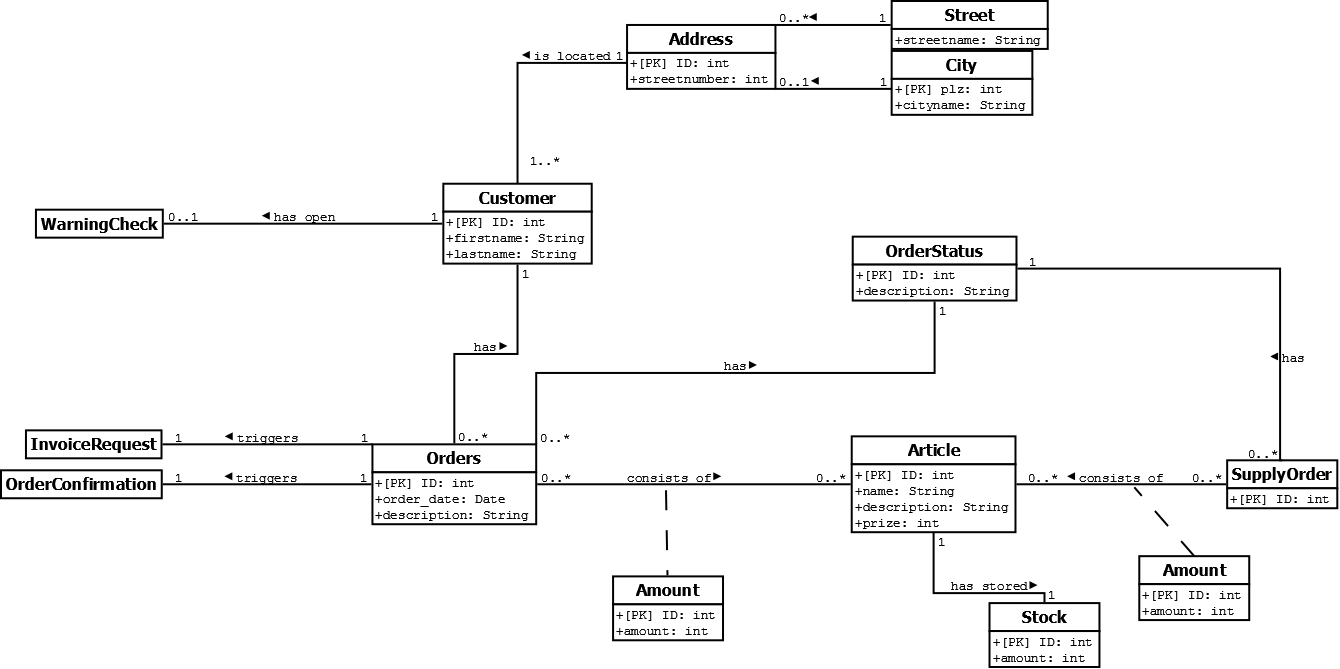
\includegraphics[width=1.0\linewidth]{Images/datamodel}
	\caption{Datenmodel}
	\label{fig:datamodel}
\end{figure}
Die Datenbank ist funktional aufgebaut und befolgt die ersten 3 Normalformen. Die Anbindung von Umsystemen sind im Datenmodell bereits abgebildet, sind jedoch nicht in der Datenbank vorhanden. Die abgebildeten Umsysteme sind WarningCheck, InvoiceRequest und OrderConfirmation.
